\documentclass[thesis.tex]{subfiles}

\chapter{Theoretical Overview and Related Works}
\section{Machine Learning}
\gls{ml} is the study of algorithms and statistical models that perform tasks without explicit instructions, but by learning and inferring from data. Machine learning algorithms produce "models" from data during their training phase, and infer the model's outputs during runtime to produce results on unseen (test) data.

Machine learning is a subfield within artificial intelligence. Most machine learning algorithms attempt to solve human-centric tasks, such as visual cognition, or language understanding, etc,... Since machine learning is approximate by nature, problems that would require machine learning solutions are often NP or incomputable.

Machine learning is closely related to statistics. A machine learning model provides prediction based on a statistical model of its training data. Although they aim to generalize to new examples, these models are still heavily bound to the training set's distribution. Understanding the statistical properties for each problem is an important step in creating accurate models.

Machine learning also has intimate ties to optimization: many learning problems are formulated as minimization of a loss function on the training set. The loss function represents the discrepancy between the model's predictions and the actual problem instances.

The key difference between machine learning and the above fields is their goals. Statistics and optimization both aim to extract results from the given (training) data, whereas machine learning is concerned with generalizing to unseen data.

\subsection{Types of learning}
There are several types of learning algorithms, including: supervised learning, unsupervised learning, semi-supervised learning, and reinforcement learning.

Supervised algorithms learn from a dataset containing both the inputs and desired outputs (labels). The trained model contains a function that associates any given input with an output, and aims to produce correct outputs for both seen and unseen data. Two sub-types of supervised learning are regression (where the output is a continuous value) and classification (where the output is one or several discrete classes). Common supervised learning algorithms include Naive Bayes classification, \gls{svm}, Decision Trees and Neural Networks. This is the most common type of machine learning, used in domains such as image classification, sentiment analysis, or speech recognition, etc,...

Semi-supervised algorithms are similar, however they are designed to handle missing labels or very small datasets, often by making heuristic assumptions for the problem.

Unsupervised algorithms, on the other hand, make use of unlabeled data, where only the input is known. Often, the goal for these models is to learn a relationship between the examples. Instead of responding to feedback, unsupervised learning algorithms identify commonalities in the data and react based on the presence or absence of such commonalities in each new piece of data. Popular unsupervised methods include k-means Clustering, and Neural Autoencoders. A major application for unsupervised learning is cluster analysis, in which entities (such as users, products, etc,...) can be classified into groups based on their features.

Finally, reinforcement learning algorithms are modeled as agents within an environment. The environment provides feedback to the agent's actions, which are interpreted as reward values. The goal in reinforcement learning is to learn a policy for the agent to perform which optimizes its reward, and ultimately achieve its task. Notable applications of reinforcement learning include self-driving cars and game-playing AIs (eg. Google's AlphaGo \cite{silver2016alphago}).

% \subsubsection{Feature extraction}
% A key phase in training any machine learning model is representing the training examples in a format suitable for the model. This process is called feature extraction.

% Feature extraction heavily relies on both the problem domain and the algorithm being used. On one hand, an example should be represented such that there's sufficient information for models to learn, while at the same time avoiding noisy features which can cause false correlation. As an example, to train a model predicting a person's height, their weight and gender could be considered good features, while their marital status would be a bad feature. On the other hand, each \gls{ml} algorithm has specific requirements and advantages in terms of input data. Naive Bayes and Decision Tree classifiers, for example, only accepts discrete values as input, while SVMs and Neural Networks only work with continuous values.

% Several common techniques are utilized in feature extraction:

% \begin{itemize}
% 	\item Normalization/Scaling: To negate the effect of uneven value ranges between features, these values are often normalized to a range between 0 to 1 (or -1 to 1), with regards to the mean value for that feature.
% 	\item Discretization: To allow discrete models to work with continuous features, discretization techniques are often applied. A common method is to split the value range into small sub-ranges.
% 	\item Embedding: Conversely, discrete features are often transformed into continuous vectors, dubbed embedding vectors. Intuitively, embedding vectors seek to approximate the relationships between their respective discrete values (eg. relations between different words). This is often achieved using some form of unsupervised learning. The most widely used form of embedding vectors is Word2Vec \cite{mikolov2013distributed} for word representation (Figure \ref{fig:word2vec}).
% \end{itemize}

% \begin{figure}[htp]
% 	\centering
% 	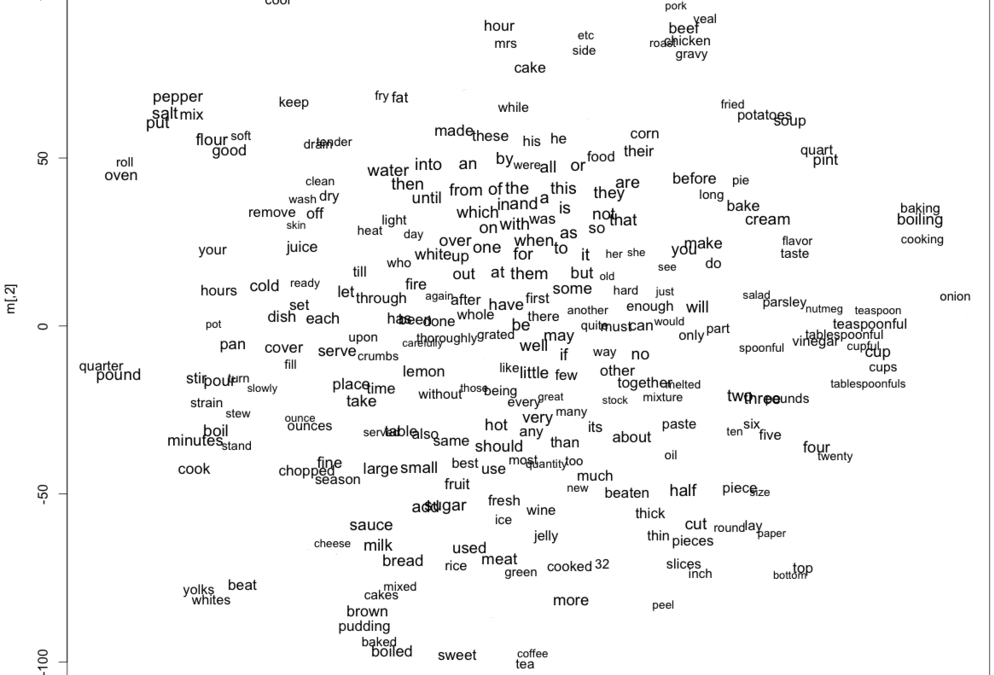
\includegraphics[width=0.9\textwidth]{word2vec.png}
% 	\caption{Visualization of word2vec embeddings}
% 	\label{fig:word2vec}
% \end{figure}

\subsection{Partitioning datasets}
Evaluating the effectiveness of \gls{ml} models differ from other algorithms and statistical models. In this section, we focus on evaluating supervised models.

Supervised \gls{ml} models are trained on a training dataset, however the goal is to produce accurate predictions on unseen data outside this training set. Hence, it's impossible to evaluate on training data, otherwise a model that "learns" by simply memorizing the training set would score perfectly, yet unusable. As such, a subset of labeled data is set aside from training as the test dataset, which only serves to evaluate the model.

Additionally, many models have hyperparameters that require selection, often by experiment. This selection should also be done on unseen data, yet it's unfair to use the test set as this simply picks out whichever parameter set that happens to fit the test distribution. Instead, a seperate validation dataset is held out for this purpose.

For large datasets, a straightforward split of 3 datasets is often made with a ratio of around 70/15/15 for training, validation and testing. In smaller datasets, an alternate approach is $k$-fold cross validation, where the entire dataset is split into $k$ equal parts (folds). Training is then performed $k$ times, each using one fold as the validation and test set, and the rest as the training set. Evaluation results are then averaged among all runs.

When splitting datasets, it can sometimes be important to maintain the distribution of classes or other feature properties in the original data. This technique is called stratified sampling, and is especially critical for datasets that are unevenly distributed.

Evaluating models on different datasets can reveal various deficiencies. A model \textit{underfits} when it achieves low metric scores on the training set, implying that the model cannot fit the problem's distribution. Using more powerful/complex models typically solves overfitting. On the other hand, a model \textit{overfits} when it achieves high metric scores on the training set, but low scores on the validation set. This means the model has learned patterns that only exists in the training data, not the desired problem's features. Regularization and data augmentation techniques are used in order to alleviate overfitting.

\subsection{Evaluation metrics}
Different metrics are used to evaluate machine learning models, depending on the problem domain. Most often, metrics focus on how accurate the model is in performing the given task, however can also include other requirements like efficiency, robustness, scalability or interpretability.

For classification models, the most common metric is accuracy, which measures the ratio of correct classifications made by the model. However, this metric can be noisy on unbalanced datasets. Specifically, if $90\%$ of the dataset belongs to class A, then a classifier that always predicts class A would have $90\%$ accuracy (!). Therefore, 3 other metrics are usually added to evaluation: precision, recall, and F1 score.

Precision measures the ratio between true positives (number of accurate predictions made by the model for one class) to all predictions in that class. Recall measures the ratio between true positives for a class and all examples labeled as that class. Finally, F1 score is the harmonic mean between precision and recall. Calculating these metrics is often done using a confusion matrix (Figure \ref{fig:confusion-mat}).

\begin{figure}[htp]
	\centering
	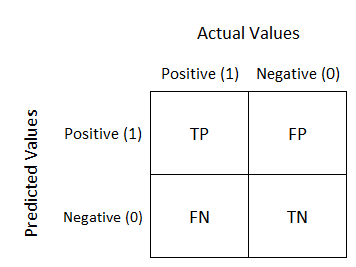
\includegraphics[width=0.5\textwidth]{confusion-mat.png}
	\caption{
		A confusion matrix\\(TP: true positive, FP: false positive, FN: false negative, TN: true negative)\protect\footnotemark}
	\label{fig:confusion-mat}
\end{figure}
\footnotetext{https://towardsdatascience.com/understanding-confusion-matrix-a9ad42dcfd62}
\FloatBarrier

More specifically, these metrics are calculated as follows:
\begin{align}
	& Precision_i = \frac{TP_i}{TP_i + FP_i}\\
	& Recall_i = \frac{TP_i}{TP_i + FN_i}\\
	& F_1^i = 2 \frac{Precision_i \cdot Recall_i}{Precision_i + Recall_i}
\end{align}

In essence, precision penalizes a model when making false predictions of the given class, while recall penalizes a model's inability to cover all examples of that class. A model that tries to "cheat" in one metric or class (like how our hypothetical "always A" model would have perfect recall for class A) invariably lower other metrics (its precision and recall for classes that aren't A would be zero), thus still having a low F1 score.

\section{Neural Networks and Deep Learning}
\subsection{Artificial Neural Networks}
Artificial neural networks (commonly referred to as neural networks) are a class of machine learning models inspired by the way biological neural systems process data.

A biological neural network is composed of a group or groups of chemically connected or functionally associated neurons. A single neuron may be connected to many other neurons and the total number of neurons and connections in a network may be extensive. Connections, called synapses, are usually formed from axons to dendrites, though dendrodendritic synapses and other connections are possible.

Artificial neural networks employ a much more simplified approximation of this process, where neurons are replaced with simple computational units that perform transformations on input data. Despite each neuron's simplicity, the amount of neurons along with their connections allow neural networks to represent incredibly complex functions.

The first neural network was proposed in 1958 by Frank Rosenblatt \cite{rosenblatt1958perceptron}, called the Perceptron. A perceptron is basically a single neuron, which consists of a set of weights $W = (w_0,..., w_n)$ and an activation function $f(x)$ (in this case the unit step function). With a continuous vector $X = (1, x_1,..., x_n)$ as input, the output of a perceptron is represented by the function:

\begin{equation}
	y = f(W \cdot X)	
\end{equation}

% \begin{figure}[htp]
% 	\centering
% 	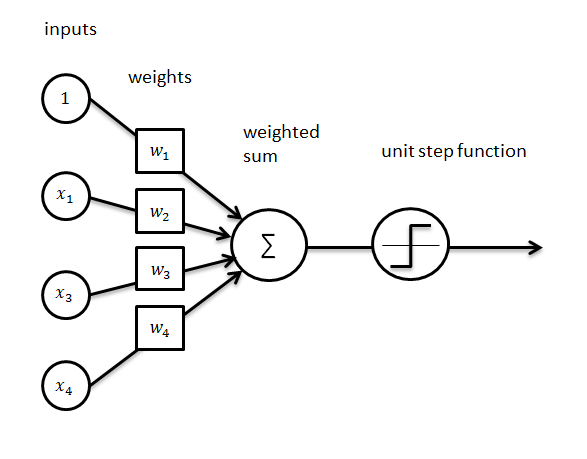
\includegraphics[width=0.5\textwidth]{perceptron.png}
% 	\caption{Diagram for a single layer binary classification perceptron\protect\footnotemark}
% 	\label{fig:perceptron}
% \end{figure}
% \footnotetext{http://ataspinar.com/2016/12/22/the-perceptron/}
% \FloatBarrier

The idea of the perceptron eventually expanded into multi layer perceptrons, or better known as artificial neural networks. Architecturally, they differ in that there are multiple "neurons" (or computational units) as opposed to one, and they are divided into layers (Figure \ref{fig:nnet}).

Three types of layer are present in a neural net: the input layer, hidden layers, and the output layer. The input layer is the representation of input data, where each unit simply contains the feature value of an example. The hidden layers are transformations performed by the network on the input, each working similarly to a perceptron. Finally, the output layer contains the output values of the network. Typically, this layer returns the values we wish to use as the final result, or values that can be inferred to produce it.

\begin{figure}[htp]
	\centering
	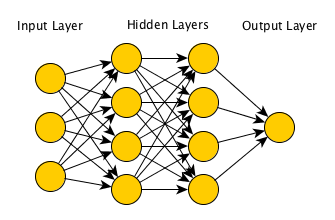
\includegraphics[width=0.5\textwidth]{nnet.png}
	\caption{Architecture of a 4-layer neural network\protect\footnotemark}
	\label{fig:nnet}
\end{figure}
\footnotetext{https://technology.condenast.com/story/a-neural-network-primer}

In this classic architecture, each neuron in layer $i$ is connected to every neuron in layer $i + 1$. As such, these networks are also referred to as fully connected networks. 

Neural networks implement 2 primary procedures: forward pass and backpropagation.

\subsubsection{Forward pass}
The forward pass is used to get output results from a neural network. Starting with an input example $X = (x_1,...,x_n)$ at the input layer, we iterate through subsequent layers one by one, calculating the output at each pass (Algorithm \ref{alg:fwd_pass}). The output for layer $i$ is defined by:

\begin{equation}
	y_i = f_i(y_{i-1} \cdot W_i)	
\end{equation}
where $f_i$ is the layer's activation function, and $W_i$ is the layer's weight matrix. The size of $W_i$ corresponds to the number of neurons at layers $i$ and $i - 1$.

In order for neural networks to represent complex, non-linear models, the activation function at each layer is often non-linear. The most widely used functions are $sigmoid$ and $tanh$ (Figure \ref{fig:sigmoid_tanh}).

\begin{figure}[htp]
	\centering
	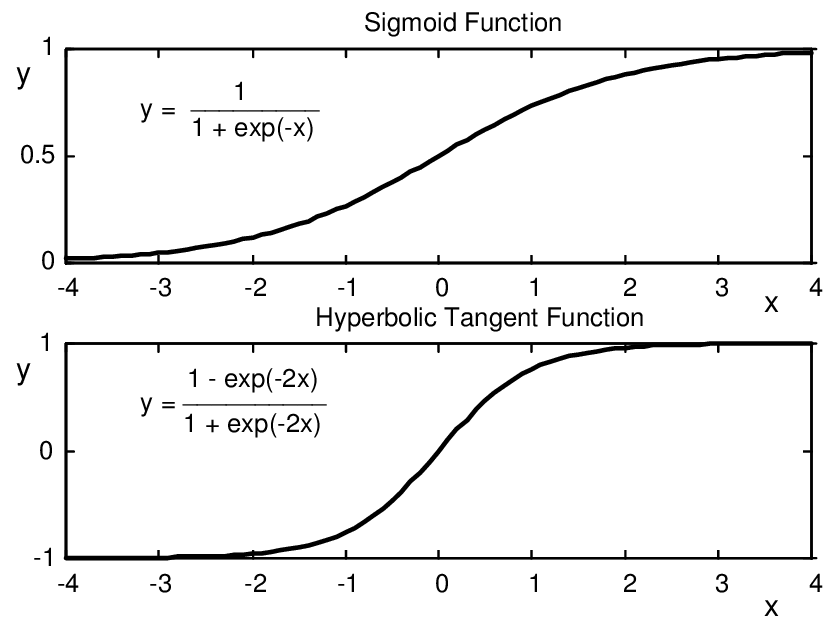
\includegraphics[width=0.5\textwidth]{sigmoid_tanh.png}
	\caption{Sigmoid and tanh activation functions\protect\footnotemark}
	\label{fig:sigmoid_tanh}
\end{figure}
\footnotetext{https://www.researchgate.net/figure/The-sigmoid-and-hyperbolic-tangent-activation-functions\_fig2\_2654867842}

\begin{algorithm}[bth]
	\SetAlgoLined
	\caption{Forward pass} \label{alg:fwd_pass}
	\Input{$X = (x_1,...,x_k)$: a set of input features\\
		$L = ((W_1, f_1),...,(W_m, f_m))$: the network's layers
		}
	\Output {
		$y_m$: the network's prediction
		$Z = (z_1,...,z_m)$: the output at each layer
	}

	$y_0 \gets X$ \\
	\For{$i \in (1...m)$} {
		$z_i \gets y_{i-1} \cdot W_i$ \\
		$y_i \gets f_i(z_i)$
	}

	\Return $y_m$, $Z$
\end{algorithm}

\subsubsection{Backpropagation}
Neural networks learn from examples using backpropagation. As the name implies, backpropagation works by tracing back from the output layer. Given a training example $X = (x_1,...,x_n)$ and the label $Y$, we first get the network's prediction $y$ using the forward pass. The general idea is to "propagate" the error signal between $y$ and $Y$ to the whole network, or in other words, update the network to decrease prediction error.

The error signal is calculated using a loss function, measuring the discrepancy between predictions and labels. Typically, regression problems employ Mean Squared Error (Equation \ref{eq:mse}), while classification problems use the Cross Entropy loss (Equation \ref{eq:cross_enp}). Other notable functions include Triplet Loss as seen with FaceNet \cite{schroff2015facenet}, and Adversarial Loss used by Generative Adversarial Networks \cite{goodfellow2014generative}.

\begin{align}
	& MSE = \frac{1}{n} \sum_{i=1}^n (y_i - Y-i)^2 \label{eq:mse}\\
	& H = - \frac{1}{n} \sum_{i=1}^n (Y_ilog(y_i) + (1-Y_i)log(1-y_i)) \label{eq:cross_enp}
\end{align}
where $n$ is the total number of examples.

In order to update the network, we need to know the values with which to update each neuron. Backpropagation finds these values for each layer $i$ using the gradient w.r.t layer $i + 1$. We start by calculating the gradient at the output layer $m$ w.r.t the loss function. Then, using the derivative chain rule, calculate the gradient at each previous layer. This is described in detail in Algorithm \ref{alg:backprop}.

\begin{algorithm}[bth]
	\SetAlgoLined
	\caption{Backpropagation} \label{alg:backprop}
	\Input{$X = (x_1,...,x_k)$: a set of input features\\
		$Y$: the correct example label\\
		$L = ((W_1, f_1),...,(W_m, f_m))$: the network's layers
		}
	\Output {
		$\Delta = (\delta_1,...,\delta_m)$: the gradient at each layer
	}

	$y, Z \gets forwardPass(X)$ \\
	$C \gets loss(y, Y)$ \\
	$\delta_m = \frac{\delta C}{\delta w_m} \odot f_m'(z_m)$ \\
	\For{$i \in (m-1...1)$} {
		$\delta_i \gets (w_{i+1}^T \cdot \delta_{i+1}) \odot f_i'(z_i)$
	}

	\Return $\Delta$
\end{algorithm}
\FloatBarrier

\subsubsection{Gradient descent}
With the gradient at each layer, we can update the network by "moving" in the opposite direction of the gradient vectors. Given a small enough step, we can guarantee that the loss function decreases. By repeating this procedure on the training dataset, the network can converge at a minimum on the loss function. This procedure is called gradient descent (Algorithm \ref{alg:grad_desc}).

\begin{algorithm}[bth]
	\SetAlgoLined
	\caption{Gradient Descent} \label{alg:grad_desc}
	\Input{$X = (x_1,...,x_k)$: a set of input features\\
		$Y$: the correct example label\\
		$L = ((W_1, f_1),...,(W_m, f_m))$: the network's layers\\
		$\gamma$: the learning rate
		}
	\Output {
		The updated network
	}
	
	\Repeat{convergence} {
		$\Delta \gets backprop(X, Y)$ \\
		$W \gets W - \gamma \Delta$
	}
\end{algorithm}
\FloatBarrier

A learning rate is specified to adjust the step for each gradient descent iteration. A high learning rate means the network is updated with large strides, which makes it susceptible to divergence at later steps. A low learning rate is more guaranteed to converge, but takes more iterations. Conventionally, the learning rate is set in the range of $10^{-2}$ to $10^{-4}$.

\begin{figure}[htp]
	\centering
	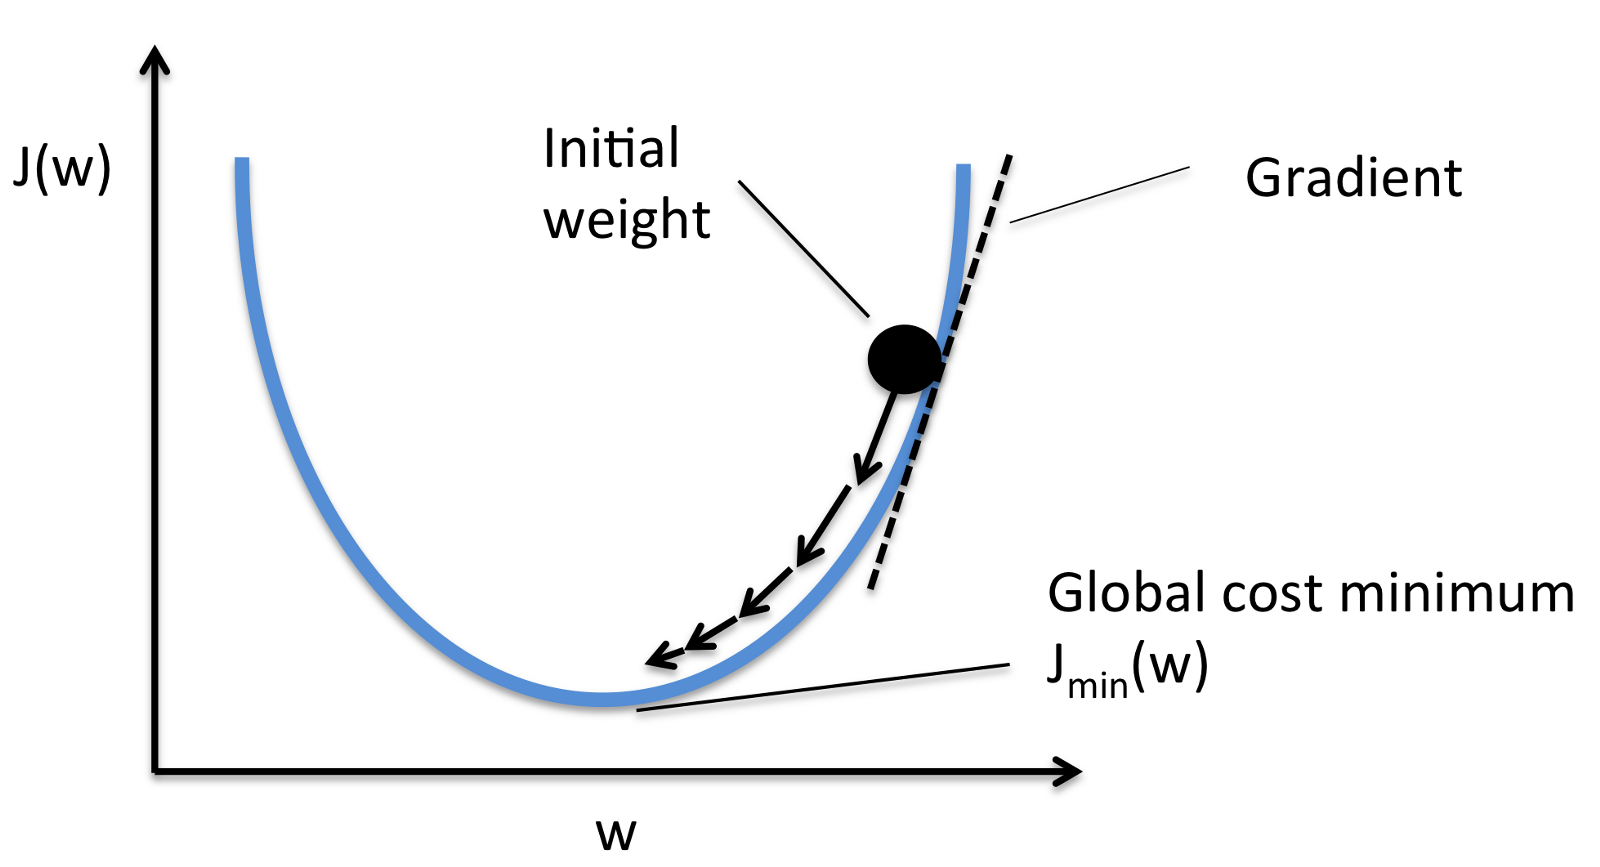
\includegraphics[width=0.7\textwidth]{gradient_descent.png}
	\caption{Gradient descent schema\protect\footnotemark}
	\label{fig:gradient_descent}
\end{figure}
\FloatBarrier
\footnotetext{https://hackernoon.com/gradient-descent-aynk-7cbe95a778da}

Gradient descent accounts for the gradient over the entire dataset. For very large datasets, this is not feasible. Minibatch gradient descent is a modified version that only updates the model on several examples at a time (one batch). This version runs in multiple "epochs", each of which goes through all batches in the dataset. Stochastic gradient descent (SGD) is a version with a batch size of 1. Stochastic and minibatch gradient descent usually requires lower learning rates and more iterations, but still consistently converges with lower memory footprints.

% \begin{figure}[htp]
% 	\centering
% 	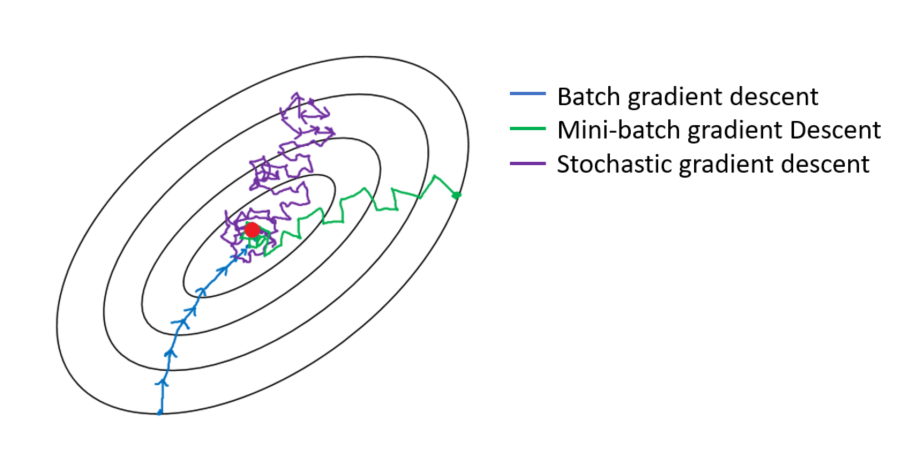
\includegraphics[width=0.7\textwidth]{gradient_descent_2.png}
% 	\caption{Convergence comparison of different gradient descent versions\protect\footnotemark}
% 	\label{fig:gradient_descent_2}
% \end{figure}
% \footnotetext{https://towardsdatascience.com/gradient-descent-algorithm-and-its-variants-10f652806a3}

Additionally, a lot of research has been conducted on adapting the learning rate during the training process, most notably resulting in several optimizers such as Adam \cite{kingma2014adam}, Adadelta \cite{zeiler2012adadelta} and RMSprop \cite{tieleman2014rmsprop}.

In general, networks with more layers and neurons can better fit the training data. However, simply increasing the number of neurons does not always result in more accurate models. Wide neural nets overfit very quickly, while networks deeper than 5-6 layers suffer from vanishing gradients. Because of these limitations, the traditional neural net architecture are only viable at a certain size.

Deep Learning techniques attempt to create larger and deeper networks while overcoming these challenges. These techniques include network architectures, optimizers, activation functions, etc,... In the next section, we look into Convolutional Neural Networks, one of the most impactful models in Deep Learning.

\subsection{Convolutional Neural Networks}
\gls{cnn} was first designed to work with images. Their architecture addresses a key problem when using ANNs to process images, as the input size can be very large (eg. 200 x 200 x 3), which quickly leads to huge, expensive networks that overfit the data.

A typical CNN is constructed from several components:

The INPUT layer is the same as a fully connected network, which holds the input features.

The CONV (convolution) layer is the core building block of a Convolutional Network (Figure \ref{fig:conv}). Its parameters consist of a set of learnable filters. Filters are small spatially (along width and height), but extends through the full depth of the input volume. For example, a typical filter on a first layer of a ConvNet might have size 5x5x3 (i.e. 5 pixels width and height with 3 color channels). During the forward pass, we slide/convolve each filter across the width and height of the input volume and compute dot products between the filter and the input at any position. As the filter slides across the input volume, it produces a 2-dimensional activation map that representing its responses at every spatial position. Intuitively, the network will learn filters that activate when they see some type of visual feature such as an edge of some orientation or a color blotch, to specific, complex patterns on higher layers of the network. Activation maps from different filters are stacked along the depth dimension and produce the output volume.

\begin{figure}[htp]
	\centering
	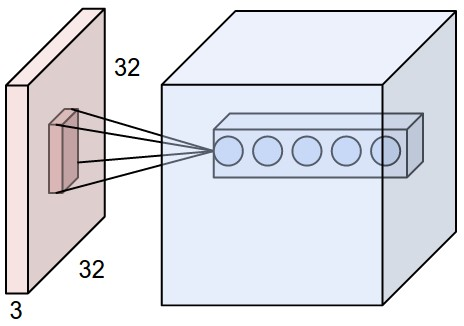
\includegraphics[width=0.4\textwidth]{conv.jpeg}
	\caption{An example convolution layer\protect\footnotemark}
	\label{fig:conv}
\end{figure}
\footnotetext{http://cs231n.github.io/understanding-cnn/}

A key difference between CONV layers and regular hidden layers is their local connectivity. Each neuron is connected to only a local region of the input volume. The spatial extent of this connectivity is a hyperparameter called the receptive field (or filter size). The extent of the connectivity along the depth axis is always equal to the depth of the input volume. It is important to emphasize this asymmetry in how we treat the spatial dimensions (width and height) and the depth dimension: The connections are local in space, but always full along the entire depth of the input volume.

The assumption made by convolution is that if a feature is a good representation for one region of the image, then it's probably good for other regions as well. As the filters convolve, the weights used for each is the same, and their gradients accumulate during backpropagation. This allows CONV layers to share weights between input regions, drastically reducing their size while still covering the entire input.

In lieu of activation functions like $sigmoid$ or $tanh$, CONV layers are usually activated using the ReLU function, with $ReLU(x) = max(x, 0)$. ReLU has several properties that helps with very deep networks:

\begin{itemize}
	\item ReLU is a non-linear function
	\item The gradient for ReLU is either 1 or 0, meaning it's not affected by vanishing gradient
\end{itemize}

One downside for ReLU is the existance of "dead neurons" whose output is negative. These neurons would have zero gradient and can no longer learn or contribute to the network. Alternative functions such as Leaky ReLU or Exponential ReLU have been proposed to overcome this.

Next, POOL (pooling) layers are used to progressively reduce the spatial size of the representation to reduce the amount of parameters and computation in the network, and hence to also control overfitting. The POOL layer operates independently on every depth slice of the input and resizes it spatially, using the MAX operation. The most common form is a pooling layer with filters of size 2x2 applied with a stride of 2 downsamples every depth slice in the input by 2 along both width and height, discarding 75\% of the activations. Every MAX operation would in this case be taking a max over 4 numbers (little 2x2 region in some depth slice). The depth dimension remains unchanged (Figure \ref{fig:maxpool}).

\begin{figure}[htp]
	\centering
	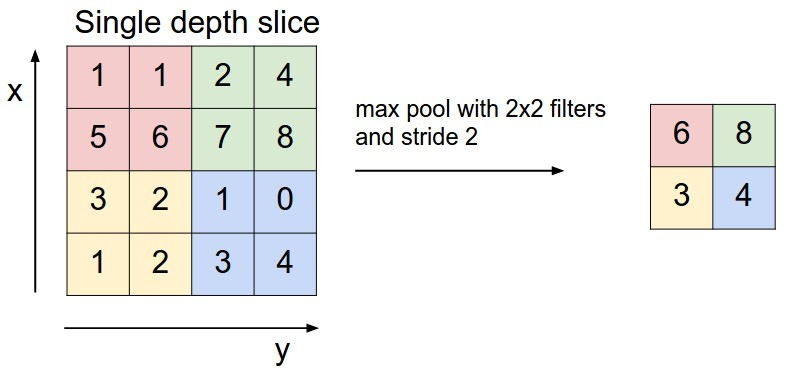
\includegraphics[width=0.6\textwidth]{maxpool.jpeg}
	\caption{An example of max pooling\protect\footnotemark}
	\label{fig:maxpool}
\end{figure}
\footnotetext{http://cs231n.github.io/understanding-cnn/}

In addition to max pooling, the pooling units can also perform other functions, such as average pooling or even L2-norm pooling. Average pooling was often used historically but has recently fallen out of favor compared to the max pooling operation, which has been shown to work better in practice.

CNNs are constructed using "blocks" of (CONV, ReLU, POOL) layers of different sizes, and finally followed by several fully connected layers to produce output results if needed (eg. classification result). VGGNet \cite{Simonyan14c} is a very effective network that follows this architecture.

Later architectures introduce more complex, non-linear ordering of convolution blocks to facilitate learning. ResNet \cite{he2016resnet}, for example, introduces skip connections (forming what's called "residual blocks") between convolution blocks.

\subsection{Object Detection with Convolutional Neural Networks}
ConvNets have been successfully applied to many computer vision problems, the most common being classification in which application is quite straightforward (using fully connected layers as the output layer). For object detection, modeling the problem's inputs and outputs with CNNs is somewhat more complex. Two types of model have been proposed and extensively researched to varying results: two-stage detection and single-stage detection.

Two-stage detection splits the problem into two subtasks: finding \glspl{roi} where there may be objects, then locating and classifying the single object within each region. The tasks are split out to handle the varying number of objects within each image. Faster R-CNN \cite{ren2015faster} is a good example of a two-stage detector. The input image is put through convolution layers to produce the initial feature map. Then, a small ConvNet is used to generate the \glspl{roi}, called the Region Proposal Network. Because \glspl{roi} can have arbitrary sizes, they are reshaped using an \gls{roi} Pooling layer. \gls{roi} pooling works similarly to max pooling, but instead of the whole feature map, it takes the feature map segment corresponding to each \gls{roi}, divides it into $m \times n$ section and performs max pooling on those sections to produce the $m \times n$ output. In essence, \gls{roi} pooling squashes \glspl{roi} of different sizes into uniform representations of their strongest signals. Afterwards, each \gls{roi} map is put through a classifier feedforward network to generate the class label. The loss function for the network is the sum of the classification loss for each correctly predicted region, and the regression loss for each predicted box.

In contrast, one-stage detectors model the problem as classifying each subregion on the image as either one of the pre-defined class (foreground) or no class at all (background). YOLO \cite{redmon2016you} and SSD \cite{liu2016ssd} are both good examples of one-stage detectors. Both architectures define multiple overlapping boxes on the feature map region. The network then learns how to correctly classify each of these boxes into the correct class, as well as the offset to the default position. Overlapping boxes of the same class are combined into a single bounding box using a procedure called Non-Maximum Suppression.

\gls{nms} is a procedure that takes a series of overlapping bouding boxes as input, and outputs the pruned list of non-overlapping boxes. \gls{nms} achieves this by prioritizing boxes with the lowest bottom-right corner, and removing any overlapping box over a predefined threshold.

For both types of detector, the model needs to pinpoint the coordinates for each bounding box. Although networks like Faster R-CNN can accomplish this by simply using the offset from a $(0, 0)$ root, this creates bias for larger boxes. Instead, fixed anchor boxes are used as base for the offsets. To best reduce bias, the anchors' shapes and ratios should cover the range of desired image shapes.

Several metrics are introduced to measure object detectors' performance. \gls{iou} is commonly used to measure box location accuracy. Given a predicted bounding box and a ground truth box, \gls{iou} is computed as the ratio between their intersection area and their union area:
\begin{equation}
	IoU = \frac{S_{overlap}}{S_{union}}
\end{equation}
A higher \gls{iou} means the box prediction more closely matches the ground truth box.

\gls{ap} is the most common and standard metric for evaluating object detectors. Average precision is calculated by first plotting the precision-recall curve. Given a set of positive prediction of the class, sort them by confidence level. As we accumlate through the sorted list, precision fluctuates according to whether the prediction is correct, while recall increases at each correct prediction, creating a zig-zag pattern. \gls{ap} is calculated as the area-under-the-curve of this precision-recall curve.

For object detection, \gls{ap} is calculated with regards to IoU, in which predictions that overlaps a ground truth box above a certain IoU are considered positives.

\section{Computational Graphs and Deep Learning Frameworks}
\subsection{Computational Graphs}
Although they are commonly visualized as layers of neurons, neural networks are more often represented as computational graphs.

\glspl{comp_graph} are directed graphs that express a series of computations. Each node is either an input variable, or, when there are incoming edges, a function of those edges' tail nodes. Edges simply denote dependencies between nodes (eg. $a = b + c$).

\begin{figure}[htp]
	\centering
	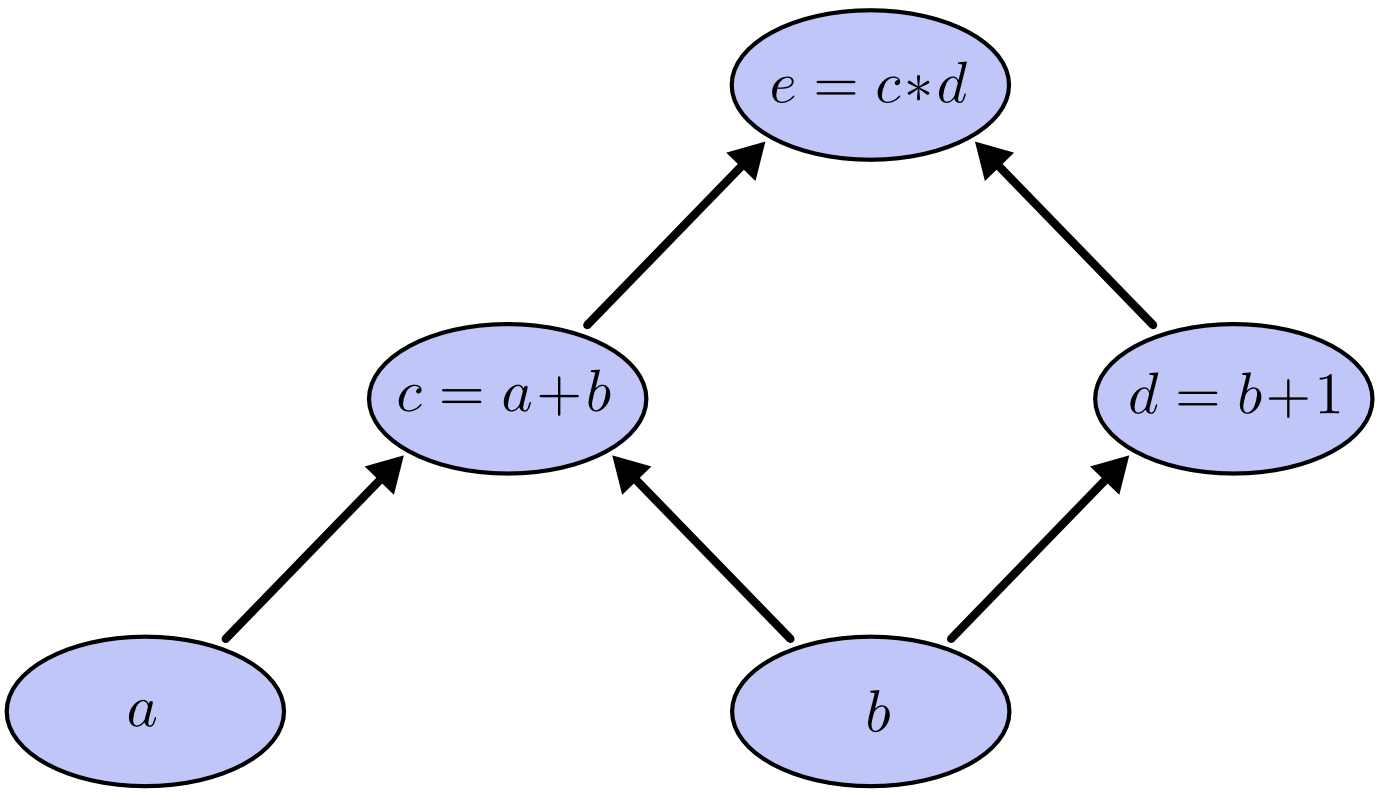
\includegraphics[width=0.4\textwidth]{cgraph1.png}
	\caption{An example computational graph with inputs $a$, $b$ and outputs $(a + b)(b + 1)$\protect\footnotemark}
	\label{fig:cgraph1}
\end{figure}
\footnotetext{http://colah.github.io/posts/2015-08-Backprop/}

It is trivial to traverse the graph from all input nodes to calculate its outputs. If we model a neural network as a series of computations (eg. $y = sigmoid(x \cdot w)$), then this corresponds to the network's forward pass. Conversely, since each node knows about its outcoming edges and operator, it can infer the gradient w.r.t each edge. In other words, we can calculate gradients at each node automatically, by traversing the graph backwards. This is immensely helpful for backpropagation, which requires the gradient for each neuron to be calculated.

The fact that neural networks can be modeled as computational graphs has several implications. Most significantly, it means that backpropagation can be done automatically, assuming each op is differentiable. This greatly reduces the amount of work required when designing network architectures, as only the forward pass need to be defined.

\subsection{Deep Learning Frameworks} \label{section:dlframeworks}
The use of computational graphs for deep learning became prevalent in part due to the multiple frameworks that leverage them for automatic gradient calculations. Two of the earliest were Theano (2010) \cite{bergstra2010theano} and Caffe (2014) \cite{jia2014caffe}, followed by Google's TensorFlow (2016) \cite{abadi2016tensorflow}, which remains the most popular framework to date. These tools define the same 2-phase workflow for running neural networks: the first phase where the computational graph is symbolically defined, and the second phase where numerical input is fed to the runtime to execute the graph.

By seperating graph definition and the actual runtime, these early frameworks can apply several optimizations during graph "compilation". This also helps improve performance, since definition is often done in the Python language, while the runtime can be written in lower-level, more performant languages (eg. C, C++,...). Finally, since the graph is finalized after compilation and is essentially data, they are portable and serializable, which helps deployment at scale.

On the other hand, compiled graphs are often criticized for their steep learning curve and being difficult to debug. Since the framework runtime completely takes over execution and even modifies the graph during optimization, it's often difficult to keep track of results and errors. This motivated the creation of dynamic graph frameworks, most notably PyTorch (2017) \cite{paszke2017pytorch} and Chainer (2015) \cite{tokui2015chainer}. These frameworks simply constructs graphs \emph{on the go}, alongside the actual calculations. This has the benefit of being easier to grasp, and operations can be transparently observed instead of obscured during execution. However, they suffer from fewer optimizations and lower portablility.

Despite their differences, static and dynamic graph frameworks have shown a tendency to overlap in recent years. Namely, TensorFlow 2.0 introduced Eager Execution, which attempts to create a smoother, dynamic experimental workflow. In contrast, PyTorch 1.0 added Script Mode in order to support compiled graphs, a feature that used to be delegated to conversion to Caffe 2. In the end, we can expect these libraries to provide both an intuitive development experience and optimized for production.

On top of these frameworks, multiple tools and interfaces have been proposed in recent years to help simplifying their workflow. High-level libraries like Keras \cite{chollet2015keras} allows intermediate users to interact more easily with TensorFlow, Theano and CNTK, while tools such as NVIDIA DIGITS create a streamlined workflow for multiple frameworks.

\section{Training Neural Networks in Parallel}
A major drawback for deep neural networks is the computational complexity of training them. LeNet (1998) \cite{lecun1998lenet}, for example, has over 100,000 parameters, while ResNet-50 (2016) \cite{he2016resnet} has 25 million. Optimizing these parameters over many iterations is very computationally intensive, and training even a small network such as LeNet could take several days on standard \glspl{cpu}.

From a parallel computing perspective, optimizing neural networks has a lot of potential optimizations. A common approach is running training examples in parallel. In each iteration, gradients are calculated for different data batches in each node, then reduced into the final update values for the model. The reduce procedure is critical in this approach, as it determines the communication overhead for each iteration. The most straightforward method would be using master nodes (often denoted parameter servers), where gradients are collected and reduced. However, this creates a bottleneck at the parameter servers themselves, and forces another level of communication if multiple parameter servers are used. 

\begin{figure}[htp]
	\centering
	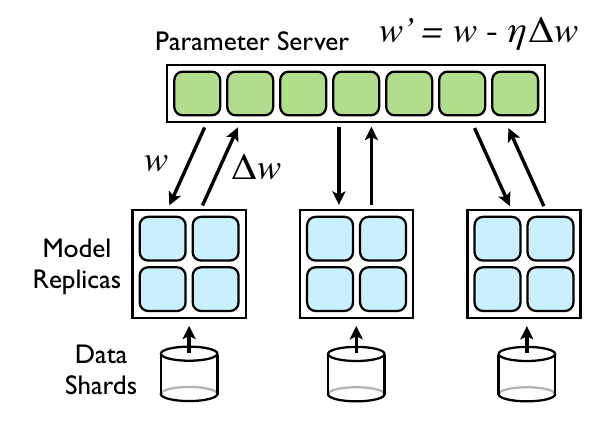
\includegraphics[width=0.5\textwidth]{allreduce.png}
	\caption{Centralized Allreduce with Parameter Server \cite{dean2012large}}
	\label{fig:allreduce}
\end{figure}

A more efficient method called "Ring Allreduce" was proposed by researchers at Baidu \cite{baiduAllreduce}. As the name suggests, this method places nodes sequentially into a "ring". When the reduce operation is called, the first node sends its gradient to node 2, where it's reduced with node 2's gradient. This result is then sent to node 3 and so on. When all nodes are reached, node 1 would contain the final gradient. We would then make another pass around the ring to update all nodes with the new gradient.

Something to take note of is the effect of this paradigm on the training results itself. Since we are running each replica on different batches, the model is essentially training with a larger batch size. Multiple works, for example \cite{chen2012pipelined}, have observed that huge batches can hinder a network's learning process, especially in early iterations. This puts somewhat of an upper limit to the scalability of this approach.

\begin{figure}[htp]
	\centering
	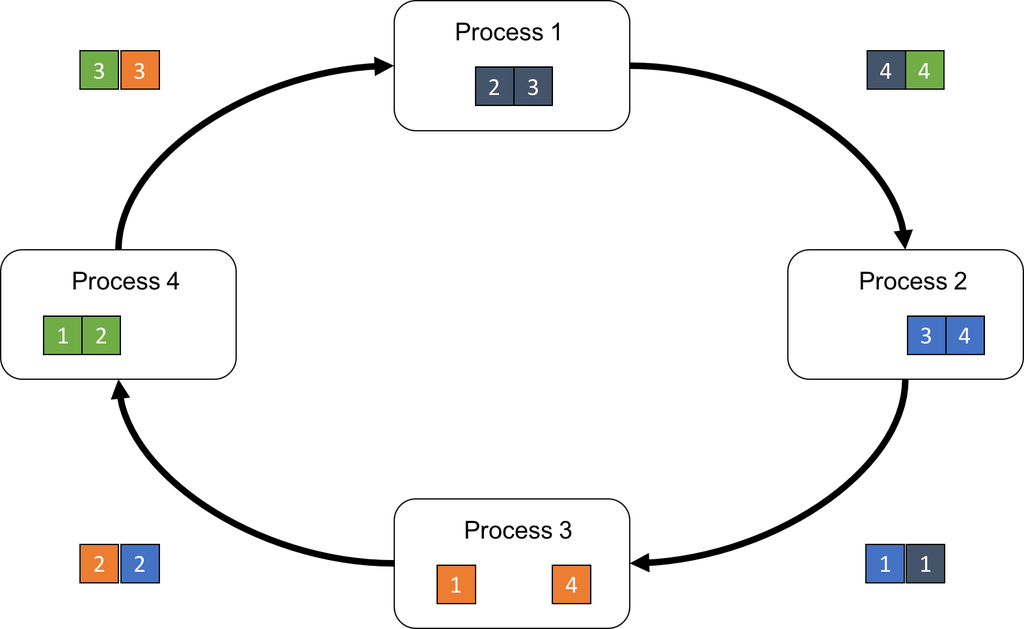
\includegraphics[width=0.6\textwidth]{ring_allreduce.png}
	\caption{Ring Allreduce\protect\footnotemark}
	\label{fig:ring_allreduce}
\end{figure}

\footnotetext{https://preferredresearch.jp/2018/07/10/technologies-behind-distributed-deep-learning-allreduce/}
\FloatBarrier

Another approach, as implemented by the authors of the DistBelief framework \cite{dean2012large}, is to distribute the network graph vertically on multiple nodes. This "striping" appproach avoids constant synchronization between nodes, but also only applicable to large, wide networks whose layers can be efficiently split.

Finally, a strategy called "pipeline backpropagation" was investigated by the authors in \cite{petrowski1993performance}. The idea is similar to striping, where the network graph is distributed across nodes. However, this method partitions the graph horizontally, where each node contains one or several full layers, forming a data pipeline. During training, each node works independently on their own data, disregarding the current state of the whole graph.

\subsection{Using Graphics Processing Units}
A breakthrough for training DNNs was the use of \glspl{gpu}, as first presented by Raina et al \cite{raina2009gpu} in 2009. Similar to graphics processing, neural networks are trained using operations on large matrices, which benefit from \glspl{gpu}' multi-core design. Since then, the toolchain for GPU-accelerated neural network has matured significantly. Libraries such as \gls{cuda}, CUDNN \cite{chetlur2014cudnn}, and high level interfaces have made training of neural networks on \glspl{gpu} trivial.

All of the frameworks mentioned in \ref{section:dlframeworks} allows execution on \glspl{gpu}, the majority of which rely on NVIDIA's CUDA and CUDNN libraries.

\subsection{Using Computing Clusters}
While \glspl{gpu} have greatly improved \gls{dnn} training speed, modern networks continue to be even more complex, along with larger training datasets. This calls for more scalable training mechanisms, particularly on multiple devices. One approach, as seen with Google's \glspl{tpu} \cite{jouppi2017datacenter}, is building custom hardware that are designed to work as clusters. Indeed, \glspl{tpu} are very efficient and performant. However, this approach is expensive and requires a lot of effort for deployment. A more compact, user-friendly approach is to make use of existing \glspl{gpu} and computer architectures. This can be done using a software layer that handles communication between GPUs/CPUs on different machines.

Support for multi-node and multi-GPU training are available in most DL frameworks, most notably TensorFlow (which utilizes Google's gRPC protocol) and PyTorch (which support several communication backends, including the popular MPI \cite{Forum:1994:MMI:898758} interface). Both implement parallelization using the data parallel approach (with Allreduce), as this is the most general solution that can apply to most neural networks.

In 2018, researchers at Uber released Horovod \cite{DBLP:journals/corr/abs-1802-05799}, a library providing a unified interface for parallel training with TensorFlow, Keras, PyTorch and MXNet. Horovod utilizes MPI for communication, and implements Baidu's Ring Allreduce. Horovod's notable feature is that it requires minimal changes to existing single-node codebases.
